% Configurazione
\documentclass[12pt, a4paper]{report}

\usepackage{graphicx}
\usepackage[table,xcdraw]{xcolor}
%\usepackage{xcolor}
\usepackage{titlesec}
\usepackage{siunitx}
\usepackage{float}
\usepackage{geometry}
\usepackage{fancyhdr}
\usepackage{verbatim}
\usepackage[italian]{babel}
\usepackage{longtable}
\usepackage{array}
\usepackage{changepage}
\usepackage{textcomp}
 \usepackage{color}
\newcolumntype{L}[1]{>{\raggedright\arraybackslash}p{#1}}
\newcolumntype{C}[1]{>{\centering\arraybackslash}p{#1}}
\newcolumntype{R}[1]{>{\raggedleft\arraybackslash}p{#1}}

\usepackage{hyperref}
\hypersetup{
    colorlinks,
    linkcolor=black,
    urlcolor=blue
}

\geometry{
  top=30mm,
  bottom=30mm,
  left=30mm,
  right=30mm,
}

\pagestyle{fancy}
\lhead{}
\lfoot{Manuale Utente}
\cfoot{}
\rfoot{\thepage}
\renewcommand{\headrulewidth}{0.4pt}
\renewcommand{\footrulewidth}{0.4pt}
\setlength{\headheight}{16pt}

\fancypagestyle{firstpage}{%
  \renewcommand{\headrulewidth}{0pt}%
  \renewcommand{\footrulewidth}{0pt}%
  \lfoot{}
  \rfoot{}
}

\graphicspath{ {immagini/} }
\definecolor{RossoUnipd}{HTML}{B5121B}
\titleformat{\chapter}{\normalfont\huge}{\thechapter.}{20pt}{\huge\textbf}

% Variabili
\newcommand\cincludegraphics[2][]{\raisebox{-0.3\height}{\includegraphics[#1]{#2}}}

\newcommand{\titolo}{Manuale Utente}

% Struttura
\begin{document}
  \thispagestyle{firstpage}
  \begin{minipage}[]{0.3\textwidth}
  
\includegraphics[width=0.8\textwidth]{logo_uni}
\end{minipage}
\begin{minipage}[]{0.6\textwidth}
  \textcolor{RossoUnipd}{
    \textbf{Università degli Studi di Padova} \\
    Laurea: Informatica \\
    Corso: Ingegneria del Software \\
    Anno Accademico: 2021/2022
  }
\end{minipage}

\bigskip

\begin{minipage}[]{0.3\textwidth}
  
\includegraphics[width=0.8\textwidth]{logo_merl}
\end{minipage}
\begin{minipage}[]{0.6\textwidth}
  Gruppo: MERL \\
  Email: \texttt{merlunipd@gmail.com}
\end{minipage}

\bigskip
\bigskip
\bigskip

  \begin{center}
  \Huge\textbf{Verbale Riunione}
\end{center}

\begin{center}
  \LARGE\textbf{01 Aprile 2022}
\end{center}

\bigskip
\bigskip
\bigskip

  \begin{center}
	\begin{tabular}{r|L{4cm}}
			\multicolumn{2}{c}{\textbf{Informazioni sul documento} } \\
			\hline
			\textbf{Versione}			& V1.0.4 \\
			\textbf{Uso}		& Esterno \\
			\textbf{Data approvazione} 			& 08/03/2022 \\
			\textbf{Distribuzione} 	&	Prof.\textit{Vardanega Tullio} \newline Prof.\textit{Cardin Riccardo} \newline \textit{Zucchetti s.p.a.} \newline Gruppo \textit{MERL} \\
	\end{tabular}
\end{center}

  \newpage
  \begin{center}
  \huge{Registro delle Modifiche}
\end{center}
\renewcommand\arraystretch{1,5}
{\centering
\begin{longtable}{|C{1.8cm}|C{2.1cm}|C{2cm}|C{2.4cm}|L{4.4cm}|}
  \hline
  \rowcolor[HTML]{036400}
  \textcolor[HTML]{FFFFFF}{\textbf{Versione}} & \textcolor[HTML]{FFFFFF}{\textbf{Data}} & \textcolor[HTML]{FFFFFF}{\textbf{Autore}}  & \textcolor[HTML]{FFFFFF}{\textbf{Verificatore}} & \textcolor[HTML]{FFFFFF}{\textbf{Modifica}}    \\ \hline
  \rowcolor[HTML]{EFEFEF}
  v2.0.0        & 04/05/2022    & Mattia Zanellato   &  -  & Approvazione \\ \hline
  \rowcolor[HTML]{C0C0C0}
  v1.0.15       & 04/05/2022    & Mattia Zanellato   &  Marco Mazzucato  & Aggiunta sottosezione "Decimo Periodo" in "Consuntivo" \\ \hline
  \rowcolor[HTML]{EFEFEF}
  v1.0.14       & 27/04/2022    & Emanuele Pase   &   Marco Mazzucato & Aggiunta sottosezione "Decimo Periodo" in "Preventivo" \\ \hline
  \rowcolor[HTML]{C0C0C0}
  v1.0.13       & 26/04/2022    & Riccardo Contin   &  Emanuele Pase  & Aggiunta sottosezione "Nono Periodo" in "Consuntivo" \\ \hline
  \rowcolor[HTML]{EFEFEF}
  v1.0.12       & 21/04/2022    & Riccardo Contin   &  Marco Mazzucato   & Aggiunta sottosezione "Nono Periodo" in "Pianificazione" e in "Preventivo" \\ \hline
  \rowcolor[HTML]{C0C0C0}
  v1.0.11       & 19/04/2022    & Emanuele Pase   &  Marco Mazzucato   & Aggiunta sottosezione "Ottavo Periodo" in "Consuntivo" \\ \hline
  \rowcolor[HTML]{EFEFEF}
  v1.0.10       & 15/04/2022    & Emanuele Pase   &  Marco Mazzucato   & Aggiunta sottosezione "Ottavo Periodo" in "Preventivo" \\ \hline
  \rowcolor[HTML]{C0C0C0}
  v1.0.9        & 13/04/2022    & Marco Mazzucato   &  Riccardo Contin   & Aggiunta sottosezione "Settimo Periodo" in "Consuntivo" \\ \hline
  \rowcolor[HTML]{EFEFEF}
  v1.0.8        & 06/04/2022    & Lorenzo Onelia   &  Riccardo Contin    & Aggiunta sottosezione "Sesto Periodo" in "Consuntivo" \\ \hline
  \rowcolor[HTML]{C0C0C0}
  v1.0.7        & 06/04/2022    & Marco Mazzucato   &   Lorenzo Onelia   & Aggiunta sottosezione "Settimo Periodo" in "Preventivo" \\ \hline
  \rowcolor[HTML]{EFEFEF}
  v1.0.6        & 06/04/2022    & Marco Mazzucato   &  Lorenzo Onelia    & Aggiunta sottosezione "Settimo Periodo" in "Pianificazione" \\ \hline
  \rowcolor[HTML]{C0C0C0}
  v1.0.7        & 31/03/2022    & Lorenzo Onelia   &  Marco Mazzucato    & Aggiunta sottosezione "Sesto Periodo" in "Preventivo" \\ \hline
  \rowcolor[HTML]{EFEFEF}
  v1.0.6        & 31/03/2022    & Lorenzo Onelia   &   Marco Mazzucato   & Aggiunta sottosezione "Sesto Periodo" in "Pianificazione" \\ \hline
  \rowcolor[HTML]{C0C0C0}
  v1.0.5        & 28/03/2022    & Marco Mamprin   &  Marco Mazzucato    & Aggiunta sottosezione "Quinto Periodo" in "Consuntivo" \\ \hline
  \rowcolor[HTML]{EFEFEF}
  v1.0.4        & 27/03/2022    & Marko Vukovic   &  Riccardo Contin    & Aggiunta sottosezione "Semaforo Rosso RTB" in "Consuntivo" \\ \hline
  \rowcolor[HTML]{C0C0C0}
  v1.0.3        & 24/03/2022    & Lorenzo Onelia  & Emanuele Pase    & Fix minori                  \\ \hline
  \rowcolor[HTML]{EFEFEF}
  v1.0.2        & 24/03/2022    & Marco Mamprin   &  Lorenzo Onelia    & Aggiunta sottosezione "Quinto Periodo" in "Preventivo" \\ \hline
  \rowcolor[HTML]{C0C0C0}
  v1.0.1        & 24/03/2022    & Marco Mamprin   &  Lorenzo Onelia    & Aggiunta sottosezione "Quinto Periodo" in "Pianificazione" \\ \hline
  \rowcolor[HTML]{EFEFEF}
  v1.0.0        & 08/03/2022    & Marko Vukovic   &  -                 & Approvazione \\ \hline
  \rowcolor[HTML]{C0C0C0}
  v0.0.17       & 04/03/2022    & Lorenzo Onelia  & Mattia Zanellato     & Aggiunta Lista di distribuzione                  \\ \hline
  \rowcolor[HTML]{EFEFEF}
  v0.0.16       & 24/02/2022     & Riccardo Contin  & Lorenzo Onelia                                & Fix finali \\ \hline
  \rowcolor[HTML]{C0C0C0}
  v0.0.15       & 23/02/2022    & Riccardo Contin   & Lorenzo Onelia                  & Pianificazione futura \\ \hline
  \rowcolor[HTML]{EFEFEF}
  v0.0.14       & 23/02/2022    & Mattia Zanellato  & Marko Vukovic                   & Aggiunta sottosezione "Quarto Periodo" in "Consuntivo" \\ \hline
  \rowcolor[HTML]{C0C0C0}
  v0.0.13       & 17/02/2022    & Riccardo Contin   & Mattia Zanellato                & Modifiche capitolo "Consuntivo" \\ \hline
  \rowcolor[HTML]{EFEFEF}
  v0.0.12       & 16/02/2022    & Mattia Zanellato  & Lorenzo Onelia                  & Aggiunto capitolo "Organigramma" \\ \hline
  \rowcolor[HTML]{C0C0C0}
  v0.0.11       & 11/02/2022    & Mattia Zanellato  & Riccardo Contin                 & Aggiunto capitolo "Mitigazione dei Rischi" \\ \hline
  \rowcolor[HTML]{EFEFEF}
  v0.0.10       & 10/02/2022    & Mattia Zanellato  & Lorenzo Onelia                  & Aggiunto capitolo "Modello di Sviluppo" \\ \hline
  \rowcolor[HTML]{C0C0C0}
  v0.0.9        & 08/02/2022    & Mattia Zanellato  & Lorenzo Onelia                  & Aggiunta sottosezione "Quarto Periodo" in "Preventivo" \\ \hline
  \rowcolor[HTML]{EFEFEF}
  v0.0.8        & 06/02/2022    & Mattia Zanellato  & Lorenzo Onelia                  & Aggiunta sottosezione "Terzo Periodo" in "Consuntivo" \\ \hline
  \rowcolor[HTML]{C0C0C0}
  v0.0.7        & 04/02/2022    & Emanuele Pase     & Marco Mamprin                   & Modifiche capitolo "Pianificazione" \\ \hline
  \rowcolor[HTML]{EFEFEF}
  v0.0.6        & 13/01/2022    & Emanuele Pase     & Marco Mamprin Riccardo Contin   & Aggiunta sottosezione "Secondo Periodo" in "Consuntivo" e sottosezione "Terzo Periodo" in "Preventivo" \\ \hline
  \rowcolor[HTML]{C0C0C0}
  v0.0.5        & 07/01/2022    & Riccardo Contin   & Lorenzo Onelia                  & Aggiunto capitolo "Introduzione" \\ \hline
  \rowcolor[HTML]{EFEFEF}
  v0.0.4        & 28/12/2021    & Riccardo Contin   & Lorenzo Onelia                  & Aggiunta sottosezione "Primo Periodo" in "Consuntivo" e sottosezione "Secondo Periodo" in "Preventivo" \\ \hline
  \rowcolor[HTML]{C0C0C0}
  v0.0.3        & 15/12/2021    & Riccardo Contin   & Marco Mamprin                   & Aggiunta sottosezione "Primo Periodo" in "Preventivo" \\ \hline
  \rowcolor[HTML]{EFEFEF}
  v0.0.2        & 11/12/2021    & Riccardo Contin   & Marco Mamprin                   & Aggiunto capitolo "Analisi dei rischi" \\ \hline
  \rowcolor[HTML]{C0C0C0}
  v0.0.1        & 08/12/2021    & Riccardo Contin   & Marco Mamprin                   & Aggiunto capitolo "Pianificazione" \\ \hline
  \rowcolor[HTML]{EFEFEF}
  v0.0.0        & 07/12/2021    & Riccardo Contin   & Marco Mamprin                   & Creata prima struttura del documento \\ \hline
\end{longtable}}

\renewcommand\arraystretch{1}

  \tableofcontents
  \newpage
  \listoffigures
  \newpage
  \listoftables

  % Capitoli
  \chapter{Introduzione}
\section{Premessa}

Il \textit{Piano di Qualifica} è un documento su cui si prevede di lavorare per l'intera durata del progetto. Molti contenuti di questo documento sono di natura instabile, come alcune metriche che non sono applicabili nella fase iniziale e che solo con il loro utilizzo pratico si può valutarne l'effettiva utilità. Anche i processi selezionati possono essere soggetti a cambiamenti, dato che possono rivelarsi insufficienti o inadeguati agli scopi del progetto e al modo di lavorare del gruppo.
Per tutte queste ragioni il documento è prodotto in maniera incrementale e suoi comntenuti iniziali sono da considerarsi incompleti.

\section{Scopo del documento}
Il \textit{Piano di Qualifica} è un documento che:
\begin{itemize}
    \item Specifica gli obiettivi
    quantitativi di qualità di prodotto e di processo;
    \item Espone le
    metodologie di controllo e le misurazioni di queste qualità tramite
    opportune metriche;
    \item Definisce quanti e quali test eseguire per verificare il corretto funzionamento
    e la qualità dei processi e del prodotto;
    \item Applica questi test e ne documenta l'esito;
    \item Crea un cruscotto di supporto che fornisce
    una visione dello stato corrente degli obiettivi.
\end{itemize}

\section{Scopo del prodotto}
Il capitolato proposto dall'azienda \textit{Zucchetti S.p.A} ha come obiettivo
quello di creare un'applicazione di visualizzazione di dati con numerose dimensioni
che permettono di rintracciare eventuali anomalie attraverso l'occhio umano. Lo
scopo del prodotto è quindi quello di fornire all'utente diversi tipi di
visualizzazione di dati in modo da rendere più veloce ed efficacie l'individuazione
di anomalie.

\section{Glossario}
Per evitare ambiguità relative alle terminoligie utilizzate è stato creato il \textit{Glossario v1.0.0} nel quale sono riportati tutti i termini importanti o con un significato particolare.
\section{Riferimenti}
\subsection{Riferimenti normativi}
\begin{itemize}
  \item \textit{Norme di Progetto v1.0.0}
\end{itemize}
\subsection{Riferimenti informativi}
\begin{itemize}
  \item \textbf{Capitolato d'appalto C5 - Login Warrior}
          \url{https://www.math.unipd.it/~tullio/IS-1/2021/Progetto/C5.pdf}
  \item \textbf{Qualità di processo}
          \url{https://www.math.unipd.it/~tullio/IS-1/2021/Dispense/T13.pdf}
  \item \textbf{Qualità di prodotto}
          \url{https://www.math.unipd.it/~tullio/IS-1/2021/Dispense/T12.pdf}
  \item \textbf{Verifica e validazione}
          \url{https://www.math.unipd.it/~tullio/IS-1/2021/Dispense/T14.pdf}
          \url{https://www.math.unipd.it/~tullio/IS-1/2021/Dispense/T15.pdf}
          \url{https://www.math.unipd.it/~tullio/IS-1/2021/Dispense/T16.pdf}
  \item \textbf{Ciclo di Deming}
          \url{https://it.wikipedia.org/wiki/Ciclo_di_Deming}
  \item \textbf{Indice di Gulpease}
          \url{https://it.wikipedia.org/wiki/Indice_Gulpease}
\end{itemize}

  \chapter{Requisiti minimi di sistema}
\section{Requisiti minimi}
    Per far funzionare l'applicazione non ci sono particolare richieste, trattandosi di una Single-page Application.

\section{Requisiti consigliati}
    Per avere un'esperienza completa nell'uso dell'applicazione si consiglia d'installare nella propria macchina i seguenti software:
    \begin{longtable}{|p{2cm}|p{2cm}|p{6cm}|}
        \hline
        \rowcolor[HTML]{036400}
        \textcolor{white}{\textbf{Software}} & \textcolor{white}{\textbf{Versione}} & \textcolor{white}{\textbf{Riferimenti per il download}} \\ \hline
            \rowcolor[HTML]{EFEFEF}
            Node.js & 16.14.2 & \href{https://nodejs.org/en/}{https://nodejs.org/en/}  \\ \hline
            \rowcolor[HTML]{C0C0C0}
            Npm & 8.x & Integrato nel download di Node.js \\ \hline
            \caption{Tabella dei requisiti consigliati}
    \end{longtable}

\section{Requisiti hardware}
    Al fine di garantire prestazioni accettabili si consiglia di soddisfare i seguenti requisiti hardware:
    \begin{longtable}{|p{3cm}|p{3cm}|}
        \hline
        \rowcolor[HTML]{036400}
        \textcolor{white}{\textbf{Componente}} & \textcolor{white}{\textbf{Versione}} \\ \hline
            \rowcolor[HTML]{EFEFEF}
            Processore & Quad-Core \\ \hline
            \rowcolor[HTML]{C0C0C0}
            RAM & 8GB \\ \hline
            \caption{Tabella dei requisiti hardware}
    \end{longtable}
    
\newpage

\section{Browser}
    I browser testati e resi compatibili con l'applicazione sono:
    \begin{longtable}{|p{2cm}|p{2cm}|}
        \hline
        \rowcolor[HTML]{036400}
        \textcolor{white}{\textbf{Browser}} & \textcolor{white}{\textbf{Versione}}\\ \hline
            \rowcolor[HTML]{EFEFEF}
            Chrome & 99\\ \hline
            \rowcolor[HTML]{C0C0C0}
            Edge & 99\\ \hline
            \rowcolor[HTML]{EFEFEF}
            Firefox & 98\\ \hline
            \rowcolor[HTML]{C0C0C0}
            Opera & 83\\ \hline
            \rowcolor[HTML]{EFEFEF}
            Safari & 15.2\\ \hline
            \caption{Tabella dei browser testati e supportati}
    \end{longtable}

  \chapter{Installazione}
Per utilizzare l'applicazione web è necessario:
\begin{itemize}
  \item Clonare il repository$_G$;
  \item Avviare il server;
  \item Avviare la web app.
\end{itemize}
\section{Clonare la repository}
\begin{itemize}
  \item Scaricare il codice come file .zip direttamente dal repository \textit{login-warrior}:
  \begin{center}
    \url{https://github.com/merlunipd/login-warrior}
  \end{center}
  oppure, avendo \textit{Git}$_G$ installato in locale, è possibile clonare il repository con il comando:
  \begin{center}
    \texttt{git clone https://github.com/merlunipd/login-warrior}
  \end{center}
  \item Localizzare da terminale la cartella in cui è stato estratto/clonato il prodotto:
  \begin{center}
    \texttt{cd percorso\LoginWarrior}
  \end{center}
\end{itemize}

\section{Avviare il server}
\begin{itemize}
  \item Entrare nella cartella \texttt{login_warrior} con i seguenti comandi:
  \begin{center}
    \texttt{cd src}
    \texttt{cd login_warrior}
  \end{center}
  \item In caso di primo avvio, per crea la cartella \texttt{node_modules} dove vengono installate tutte le dipendenza necessarie digitare:
  \begin{center}
    \texttt{npm install}
  \end{center}
  \item Per listare gli script impostati digitare (\textbf{Opzionale}):
  \begin{center}
    \texttt{npm run}
  \end{center}
  \item Per eseguire un server locale che permette l'accesso all'applicazione digitare:
  \begin{center}
    \texttt{npm run server}
  \end{center}
\end{itemize}

\section{Avviare la web app}
Dopo aver avviato il server come spiegato nel passo precedente, l'applicazione sarà disponibile aprendo l'indirizzo fornito dal terminale:
\begin{figure}[ht]
	\centering
	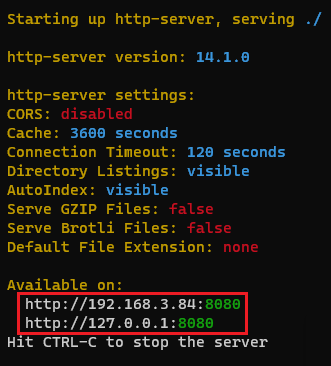
\includegraphics[width=200px]{server.png}
	\caption{Avvio dell'applicazione}
  \end{figure}

  \chapter{Istruzioni all'uso}
Il seguente capitolo fornirà tutte le spiegazioni per il corretto utilizzo del prodotto.

\section{Home}
Questa è la prima schermata disponibile dell'applicazione. Qui è possibile caricare i dati sotto forma di dataset o di sessione salvata in precedenza.

\begin{figure}[H]
    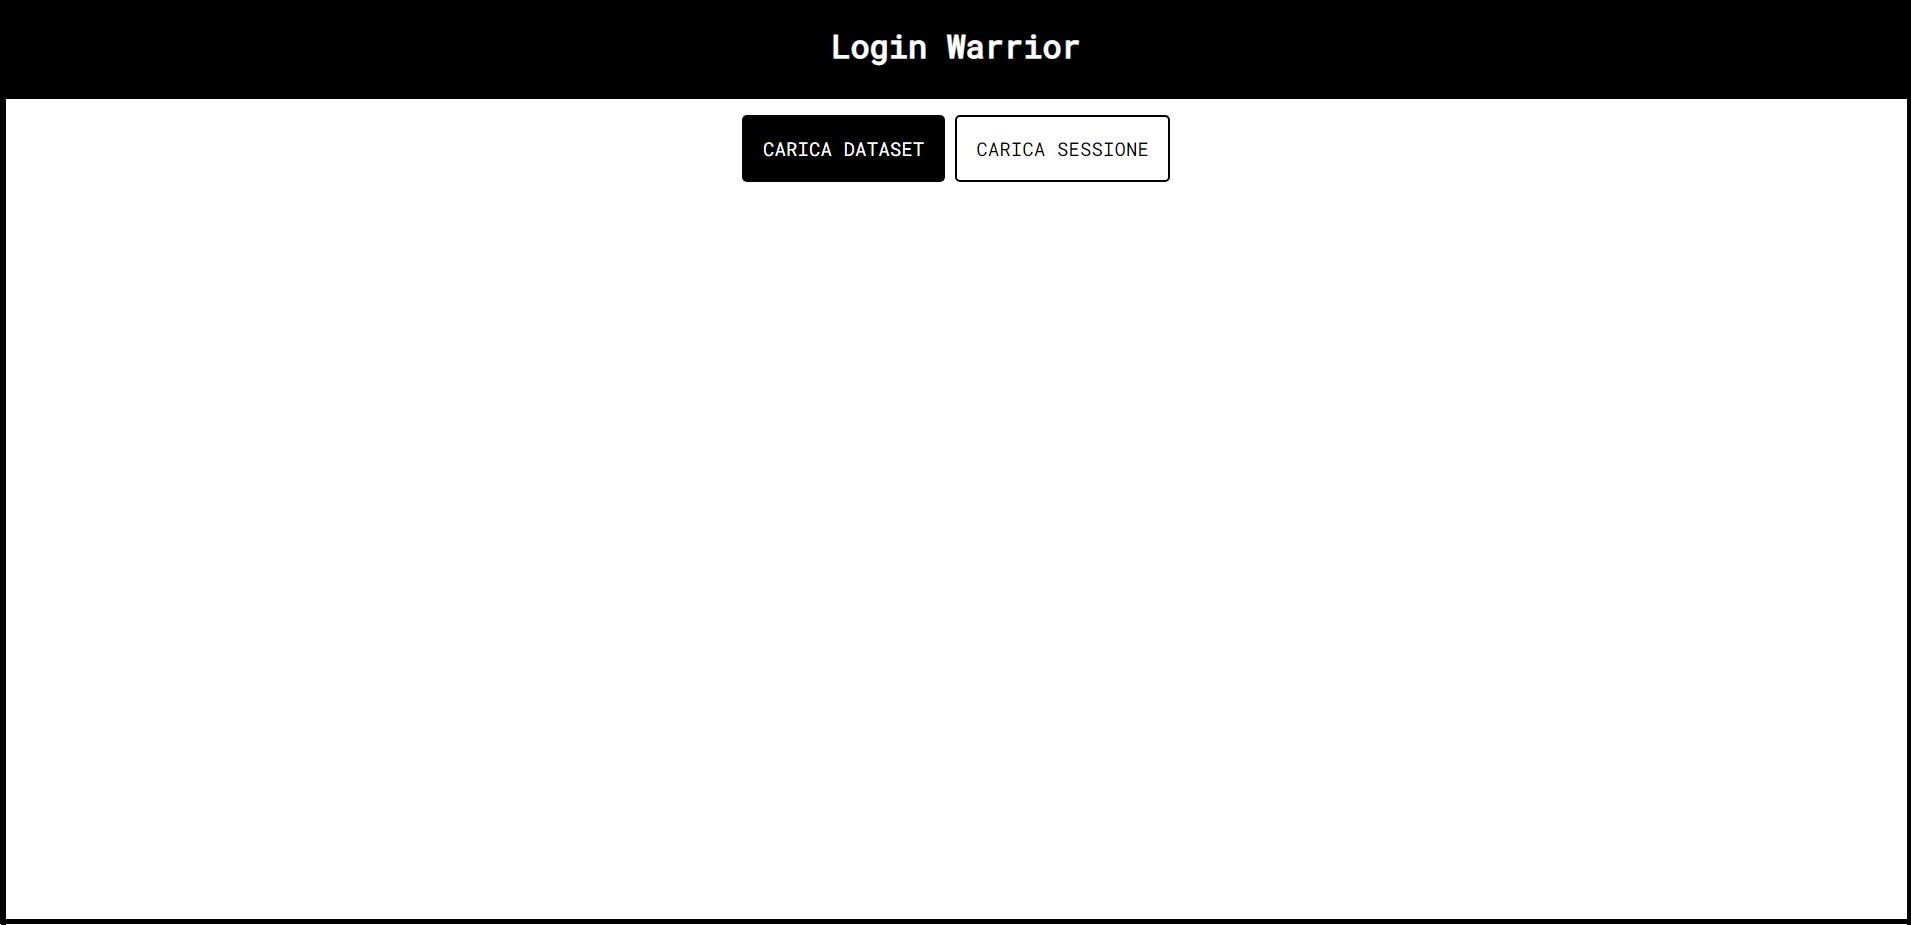
\includegraphics[width=1.0\textwidth]{Home.jpg}
    \caption{Screenshot della Home}
\end{figure}

\subsection{Carica dataset}
Cliccando su "Carica dataset" comparirà una finestra di dialogo che ci permetterà di caricare il dataset. Seleziona quindi il file in formato .csv desiderato e poi clicca su "Apri" per caricare il file.

\begin{figure}[H]
    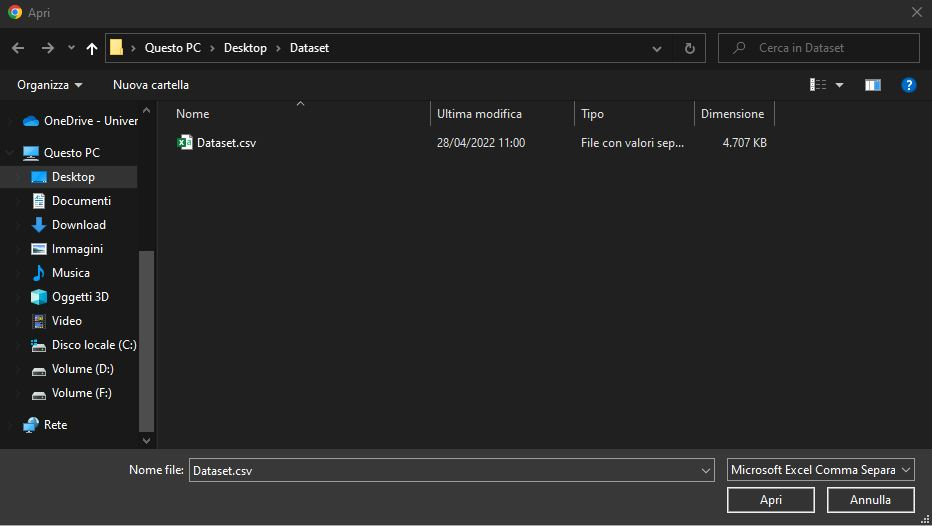
\includegraphics[width=1.0\textwidth]{BottoneDataset.jpg}
    \caption{Screenshot della finestra di dialogo per il caricamento del dataset}
\end{figure}

Dopo aver caricato il dataset comparirà una lista dei grafici disponibili.
Si potrà scegliere tra vari tipi di:
\begin{itemize}
  \item \textit{Scatter Plot};
  \item \textit{Parallel Coordinates};
  \item \textit{Sankey Diagram}.
\end{itemize}

\begin{figure}[H]
    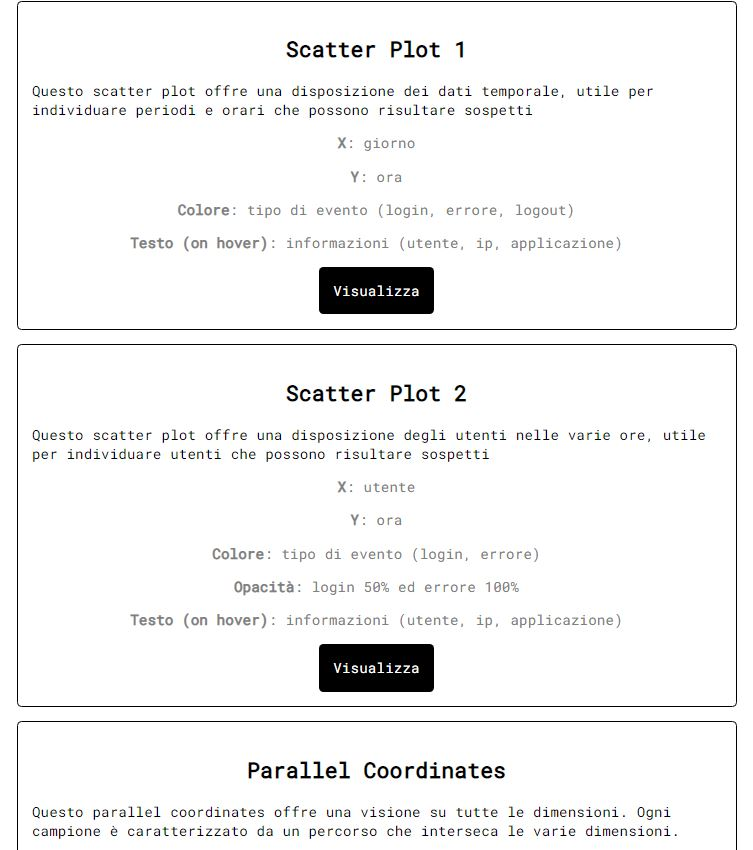
\includegraphics[width=1.0\textwidth]{ListaGrafici.jpg}
    \caption{Screenshot della lista dei grafici}
\end{figure}
Successivamente per visionare il grafico desiderato basterà premere il relativo bottone "Visualizza".

\subsection{Carica sessione}
Cliccando su "Carica sessione" comparirà una finestra di dialogo che ci permetterà di caricare i dati di una sessione salvata in precedenza. Seleziona quindi il file in formato .json desiderato e poi clicca su "Apri" per caricare il file.

\begin{figure}[H]
    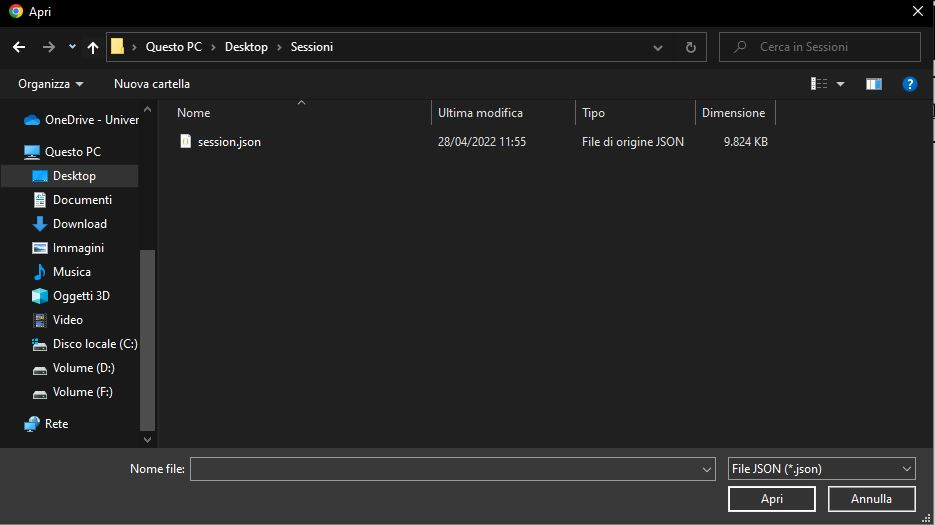
\includegraphics[width=1.0\textwidth]{BottoneSessione.JPG}
    \caption{Screenshot della finestra di dialogo per il caricamento della sessione}
\end{figure}

Dopo aver caricato la sessione nel sistema si potrà proseguire il lavoro da dove era stato salvato.

\begin{figure}[H]
    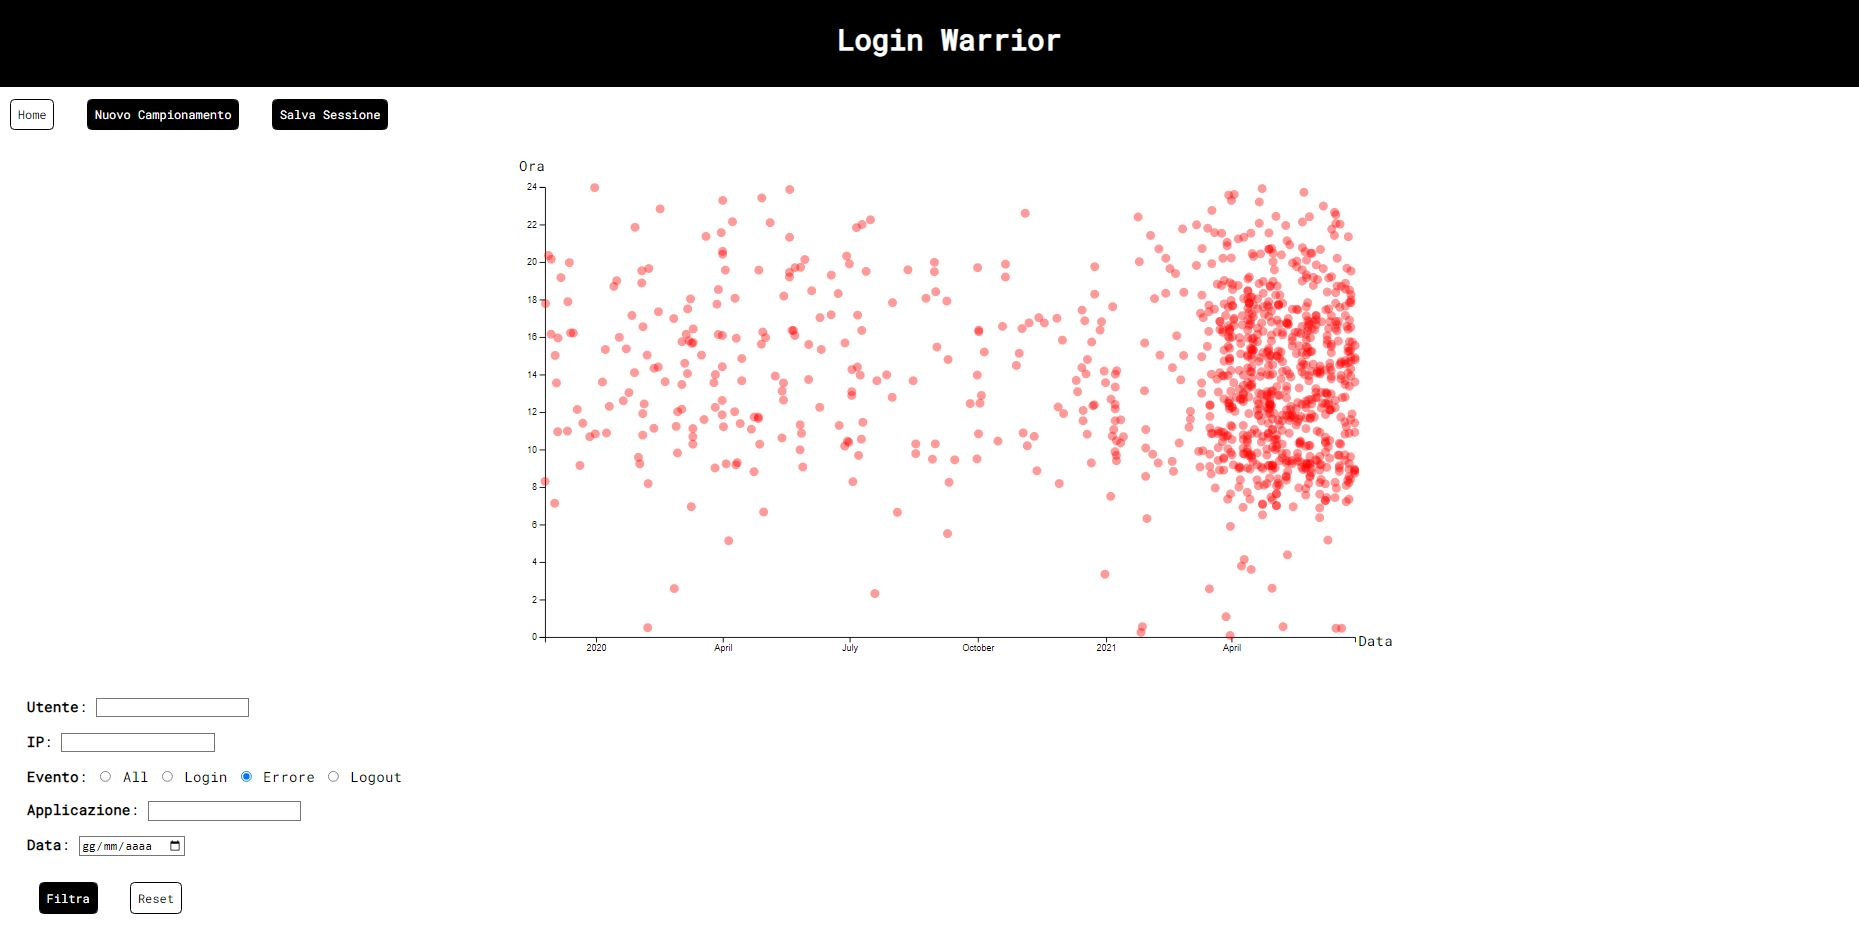
\includegraphics[width=1.0\textwidth]{CaricamentoSessione.JPG}
    \caption{Screenshot della sessione caricata}
\end{figure}

\section{Bottoni}
Nella pagina di visualizzazione del grafico, sono disponibili tre bottoni. Questi si trovano nell'estremo superiore sinistro della pagina.

\begin{figure}[H]
    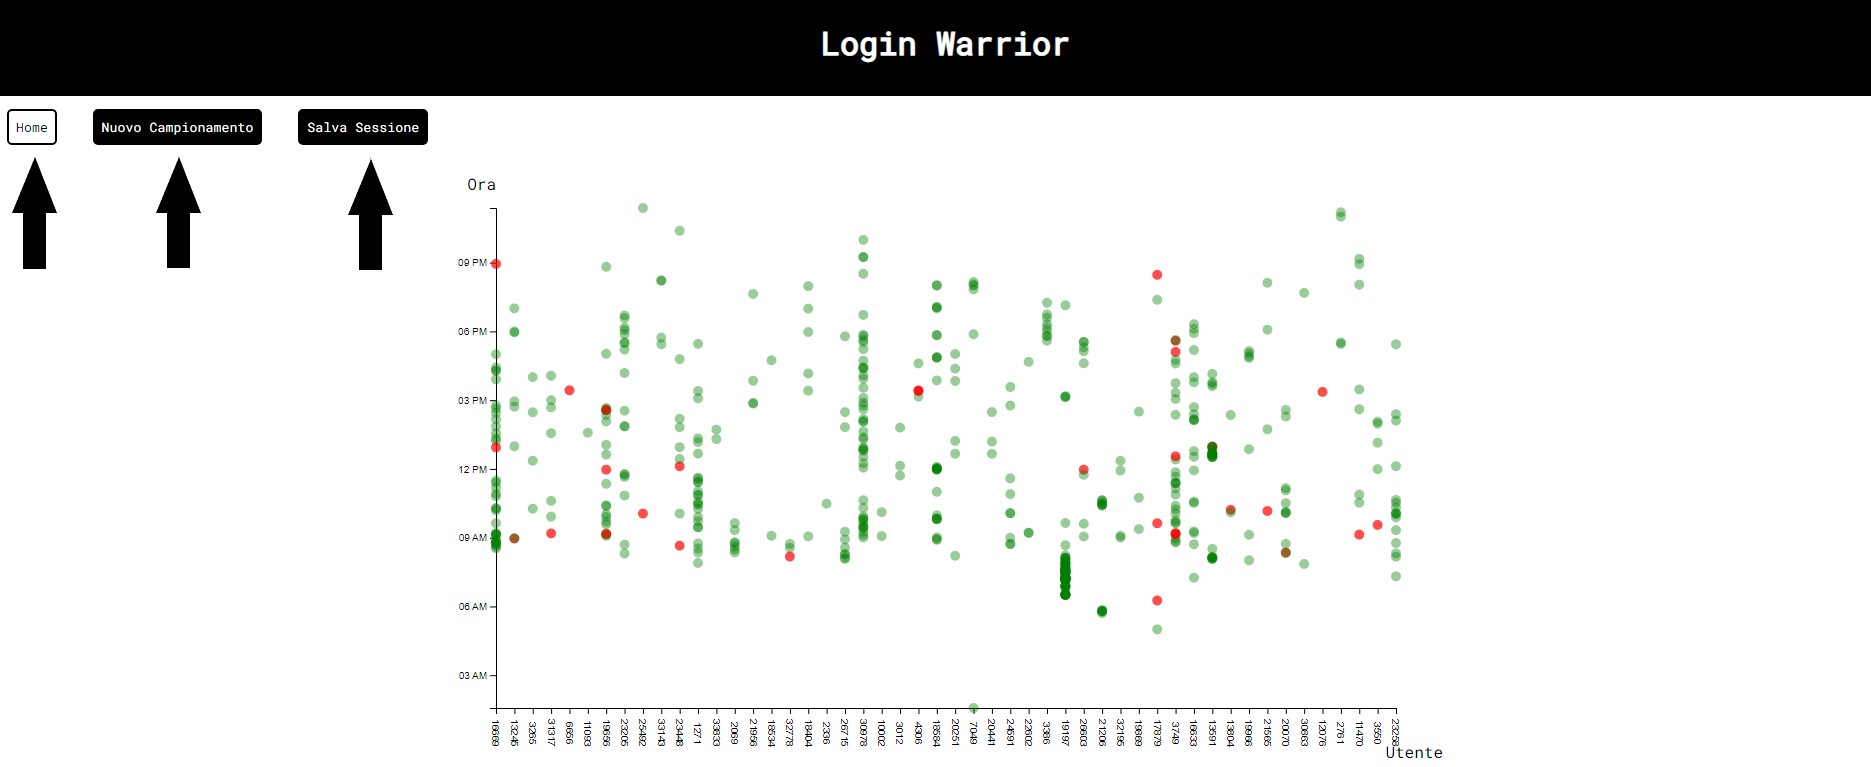
\includegraphics[width=1.0\textwidth]{Bottoni1.JPG}
    \caption{Screenshot che indica la posizione dei bottoni}
\end{figure}

\subsection{Bottone Home}
Questo bottone permette di ritornare alla Home in qualsiasi momento mantenendo comunque in memoria il dataset caricato, permettendo di scegliere un altra tipologia di grafico o di caricare un nuovo file.

\subsection{Nuovo Campionamento}
Ogni grafico attua un appropriato algoritmo di campionamento dei dati per permettere all'utilizzatore di avere una buona visualizzazione delle informazioni (il numero di dati potrebbe essere estremamente grande, quindi non gestibile).
Questo bottone permette di estrapolare ogni volta dei dati nuovi attraverso l'algoritmo di campionamento. Se il numero di dati del dataset è inferiore al numero massimo di dati che il grafico può visualizzare questo bottone non provoca cambiamenti.

\subsection{Salva Sessione}
Questo bottone permette di salvare la sessione corrente in tutti i suoi aspetti, compresi i filtri e dataset intero. Basterà premerlo per scaricare la sessione nel formato .json.

\section{Filtri}
In ogni grafico è possibile impostare dei filtri. Questi sono impostabili dall'estremo inferiore sinistro della pagina. Una volta inseriti i filtri desiderati occorre premere il bottone "Filtra" per applicarli. Per resettare i filtri invece occorre premere il bottone "Reset".

\begin{figure}[H]
    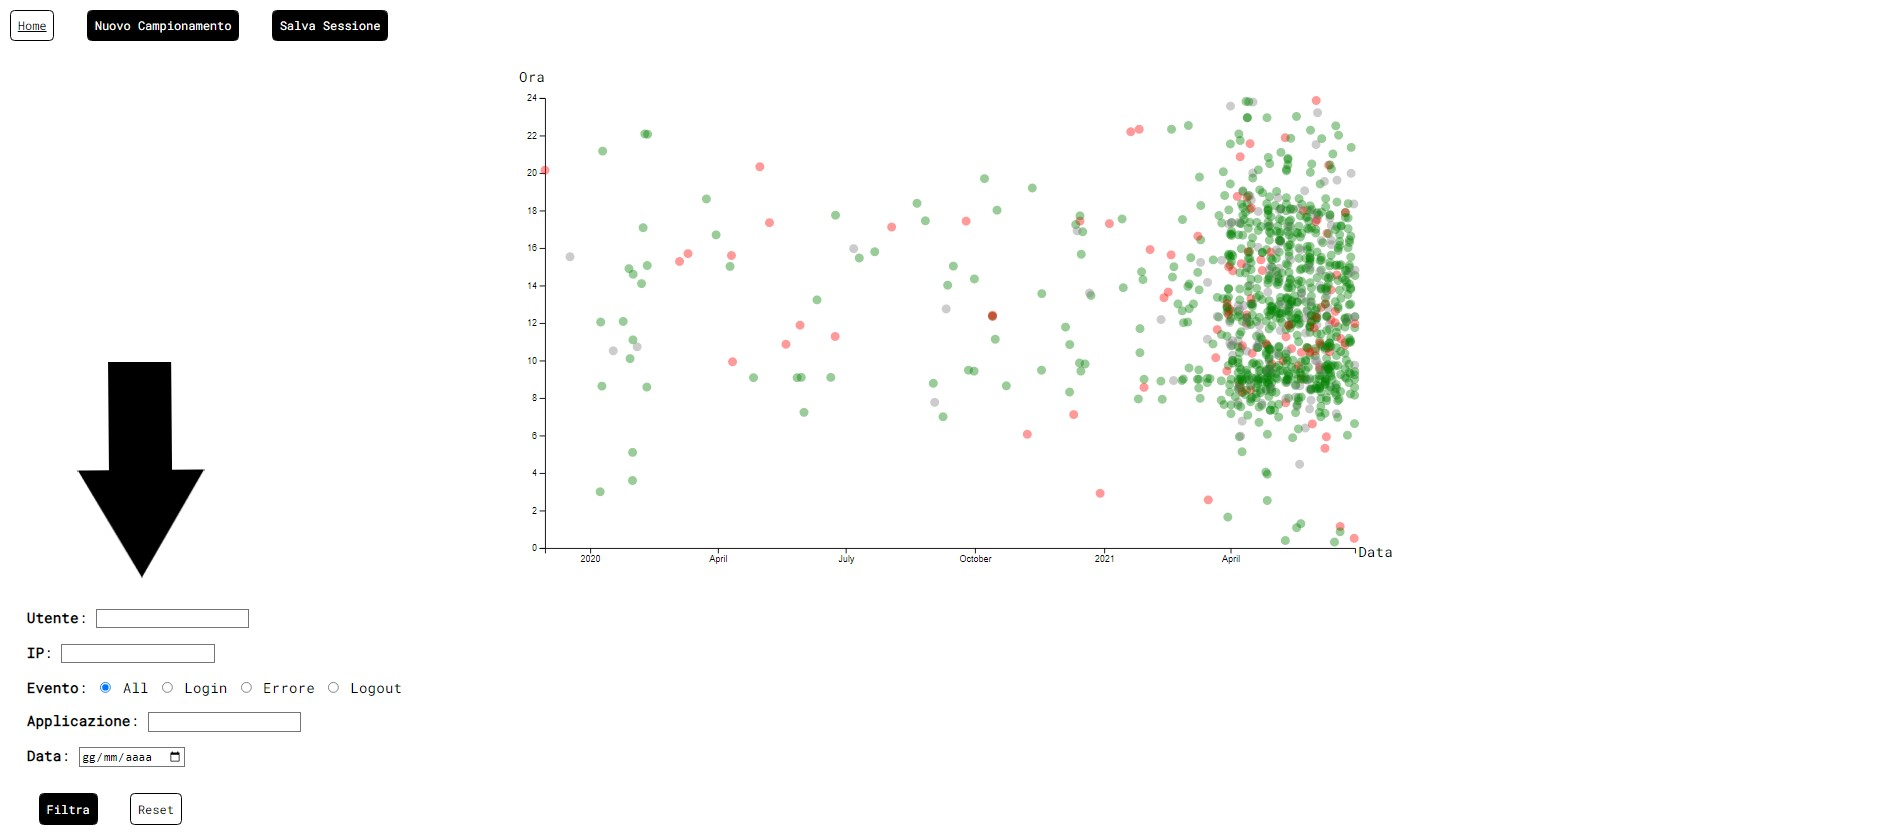
\includegraphics[width=1.0\textwidth]{Filtri.JPG}
    \caption{Screenshot che indica la posizione dei filtri}
\end{figure}

\subsection{Utente}
In questo campo è possibile inserire il numero di un utente se si vuole visualizzare il grafico contenente solo i suoi accessi.

\subsection{Ip}
In questo campo è possibile inserire un indirizzo IP se si vuole visualizzare il grafico contenente solo i suoi accessi.

\subsection{Evento}
Questo filtro permette di filtrare i dati secondo i vari tipi di evento, ovvero:
\begin{itemize}
  \item Login;
  \item Errore;
  \item Logout.
\end{itemize}

\subsection{Applicazione}
In questo campo è possibile inserire il nome di un'applicazione se si vuole visualizzare il grafico contenente solo gli accesi effettuati tramite essa.

\subsection{Data}
Qui viene fornito un calendario dal quale è possibile scegliere una data che permette di visualizzare gli accessi avvenuti in quella determinata giornata.

\section{Scatter Plot}
Il grafico \textit{Scatter Plot} permette di visualizzare ogni azione degli utenti sotto forma di punti all'interno del piano cartesiano.
Ogni evento ha un colore differente per avere una più facile visualizzazione.
Il verde indica un login effettuato con successo, il rosso un errore e il grigio un logout.
Per visualizzare le informazioni di ogni evento si dovrà posizionare il cursore al di sopra del pallino scelto. Le informazioni disponibili sono:
\begin{itemize}
  \item Ip;
  \item Numero Utente;
  \item Tipologia di evento;
  \item Data;
  \item Applicazione da dove è stata compiuta l'azione.
\end{itemize}

\begin{figure}[H]
    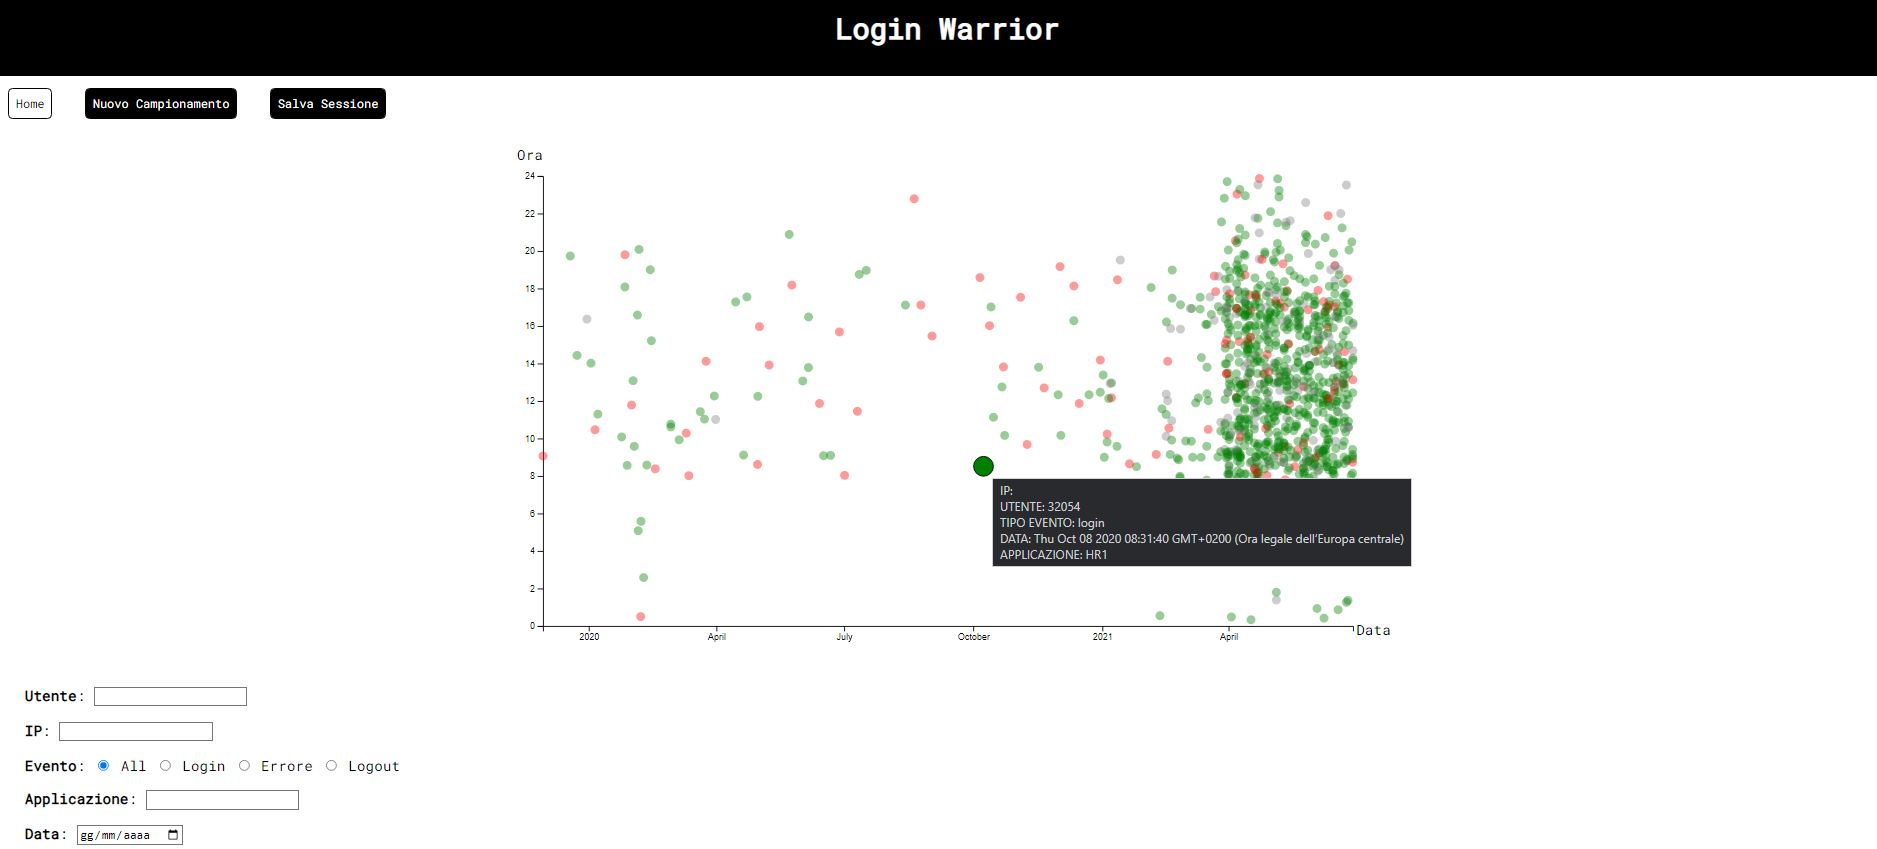
\includegraphics[width=1.0\textwidth]{VisualizzaInformazioni.JPG}
    \caption{Screenshot che mostra le informazioni di un punto}
\end{figure}

\section{Parallel Coordinates}
Il grafico \textit{Parallel Coordinates} permette di visualizzare ogni accesso sotto forma di linea.
Per visualizzare le informazioni di un particolare evento si dovrà posizionare il cursore al di sopra della linea scelta. Le informazioni disponibili sono:
\begin{itemize}
  \item Ip;
  \item Numero Utente;
  \item Tipologia di evento;
  \item Data;
  \item Applicazione da dove è stata compiuta l'azione.
\end{itemize}

\begin{figure}[H]
    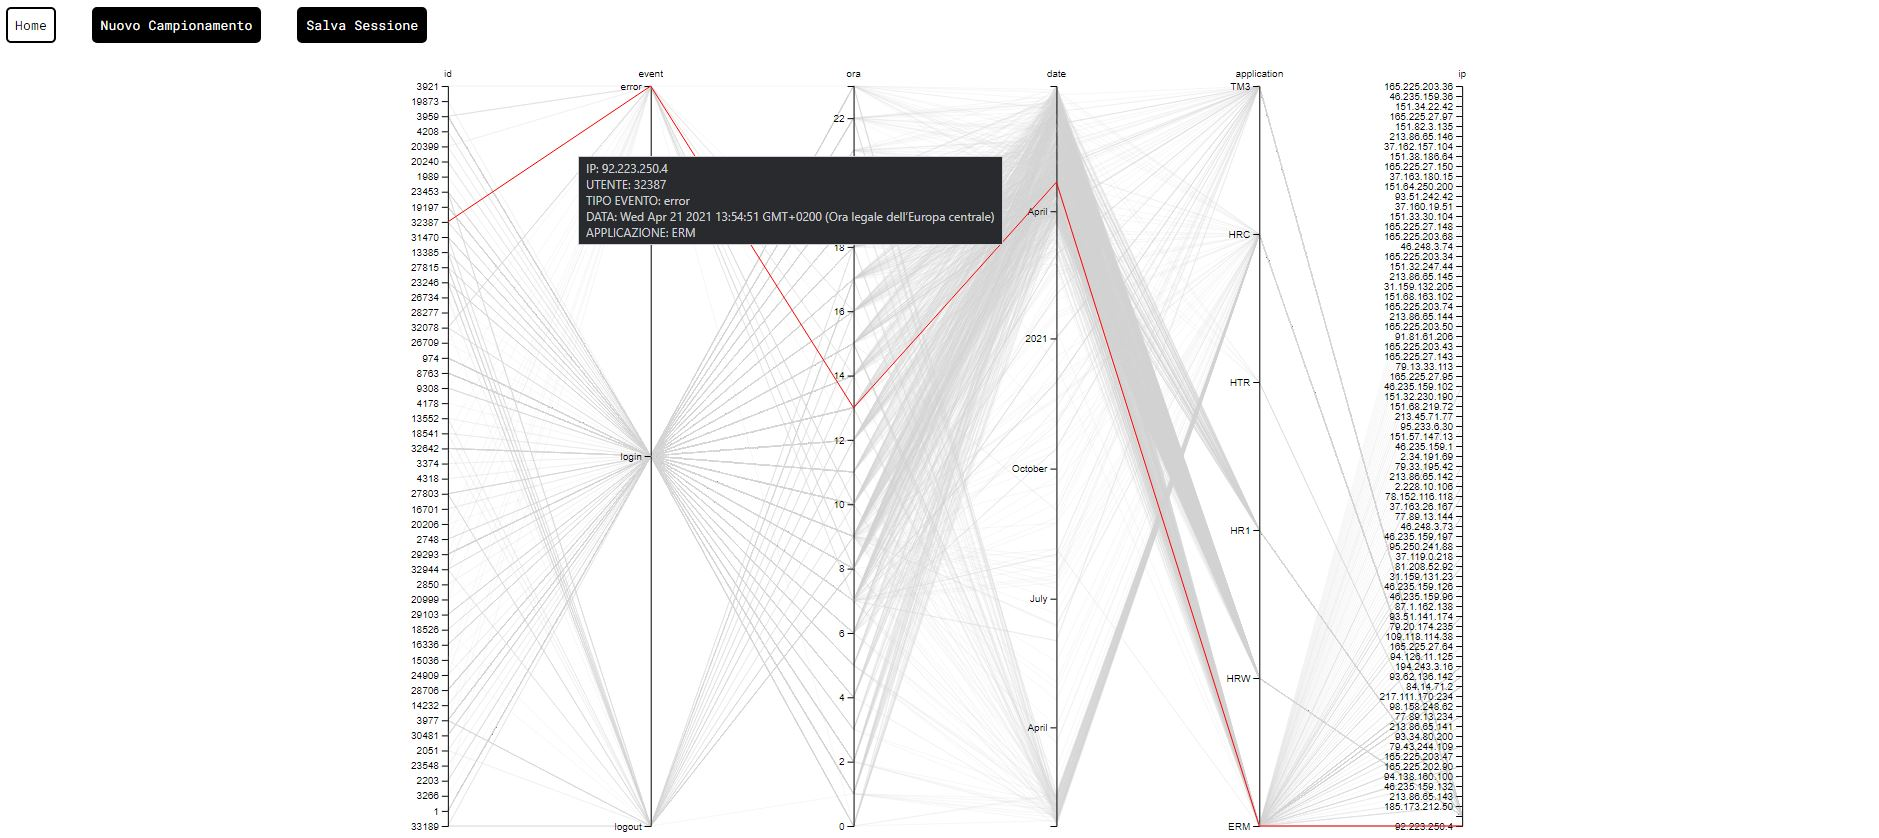
\includegraphics[width=1.0\textwidth]{Coordinates.JPG}
    \caption{Screenshot che mostra le informazioni di una linea}
\end{figure}

\section{Sankey Diagram}
Il grafico \textit{Sankey Diagram} permette di visualizzare gli eventi raggruppati in nodi.
È per esempio possibile visualizzare quanti login ci sono stati nel mese di Aprile nell'orario d'ufficio.
Per visualizzare il numero di dati che ogni nodo contiene basterà posizionare il cursore al di sopra del rettangolo colorato che indica i dati che ci interessano.

\begin{figure}[H]
    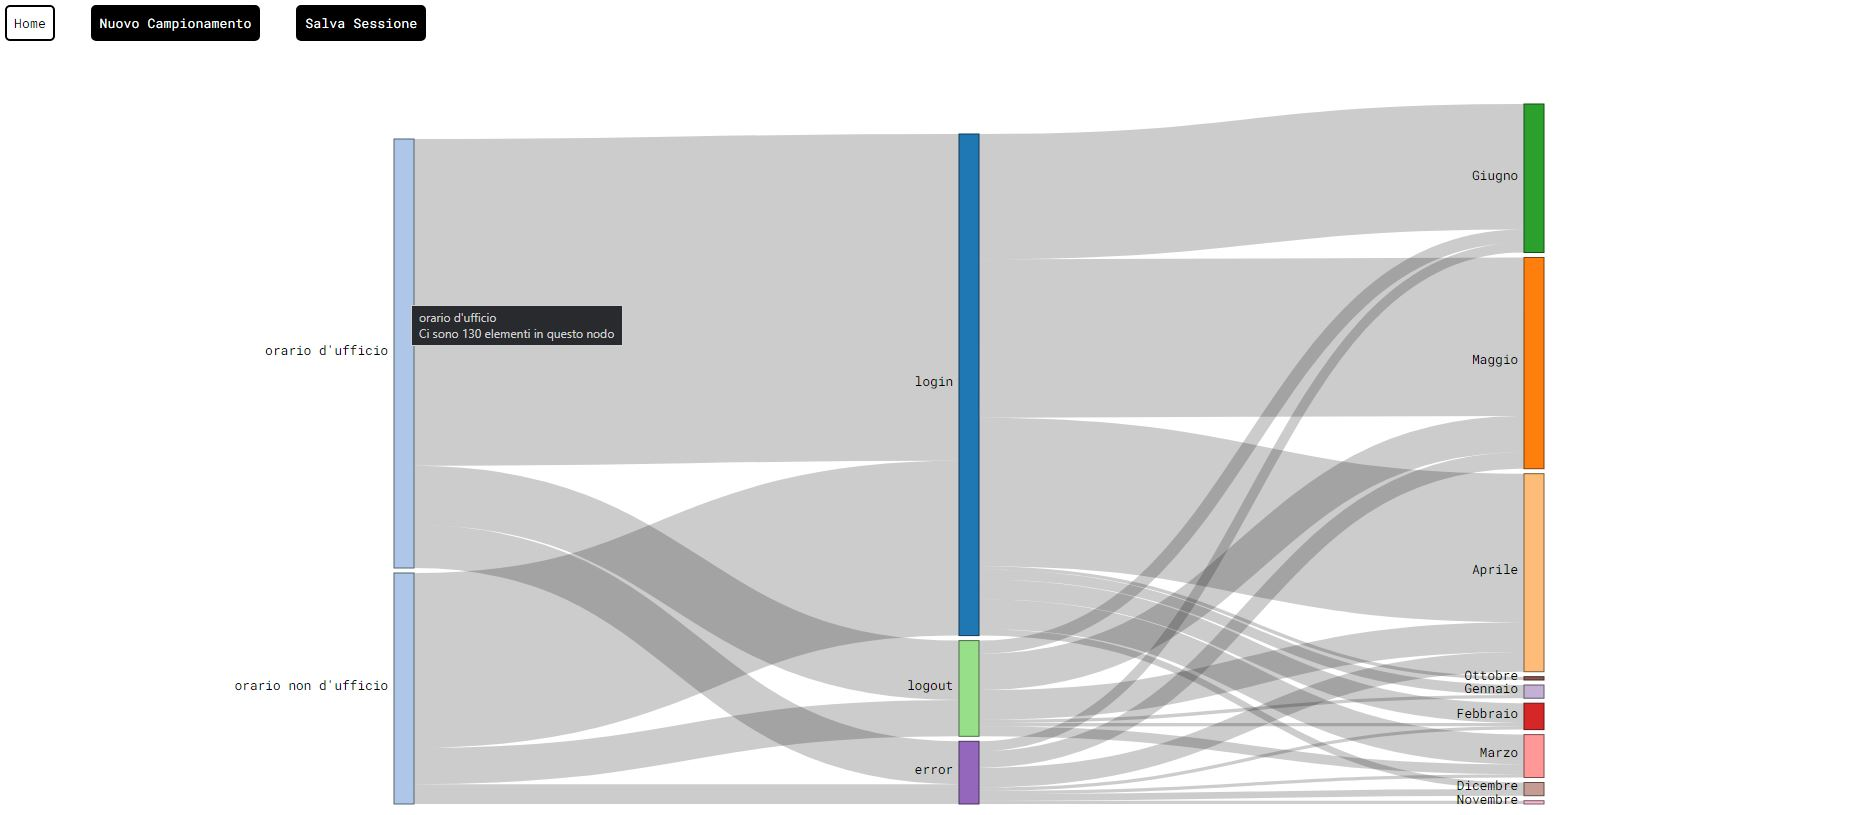
\includegraphics[width=1.0\textwidth]{Sankey.JPG}
    \caption{Screenshot che mostra le informazioni di un nodo}
\end{figure}

  \chapter{Supporto tecnico}

\end{document}
